%!TEX root=../../main.tex


\subsection{Single-source Shortest-paths}

\subsubsection{Single-node}
\autoref{fig:singleNodeSSSP} shows the average calculation times (time without initialization overhead), execution time and the normalized overhead for SSSP on the different frameworks. In these figures, Galois with 96 threads is shown. We show the impact of Galois' thread count in \autoref{sec:galois_speedup}.
\begin{figure*}[ht!]
	\begin{subfigure}{0.3\textwidth}
		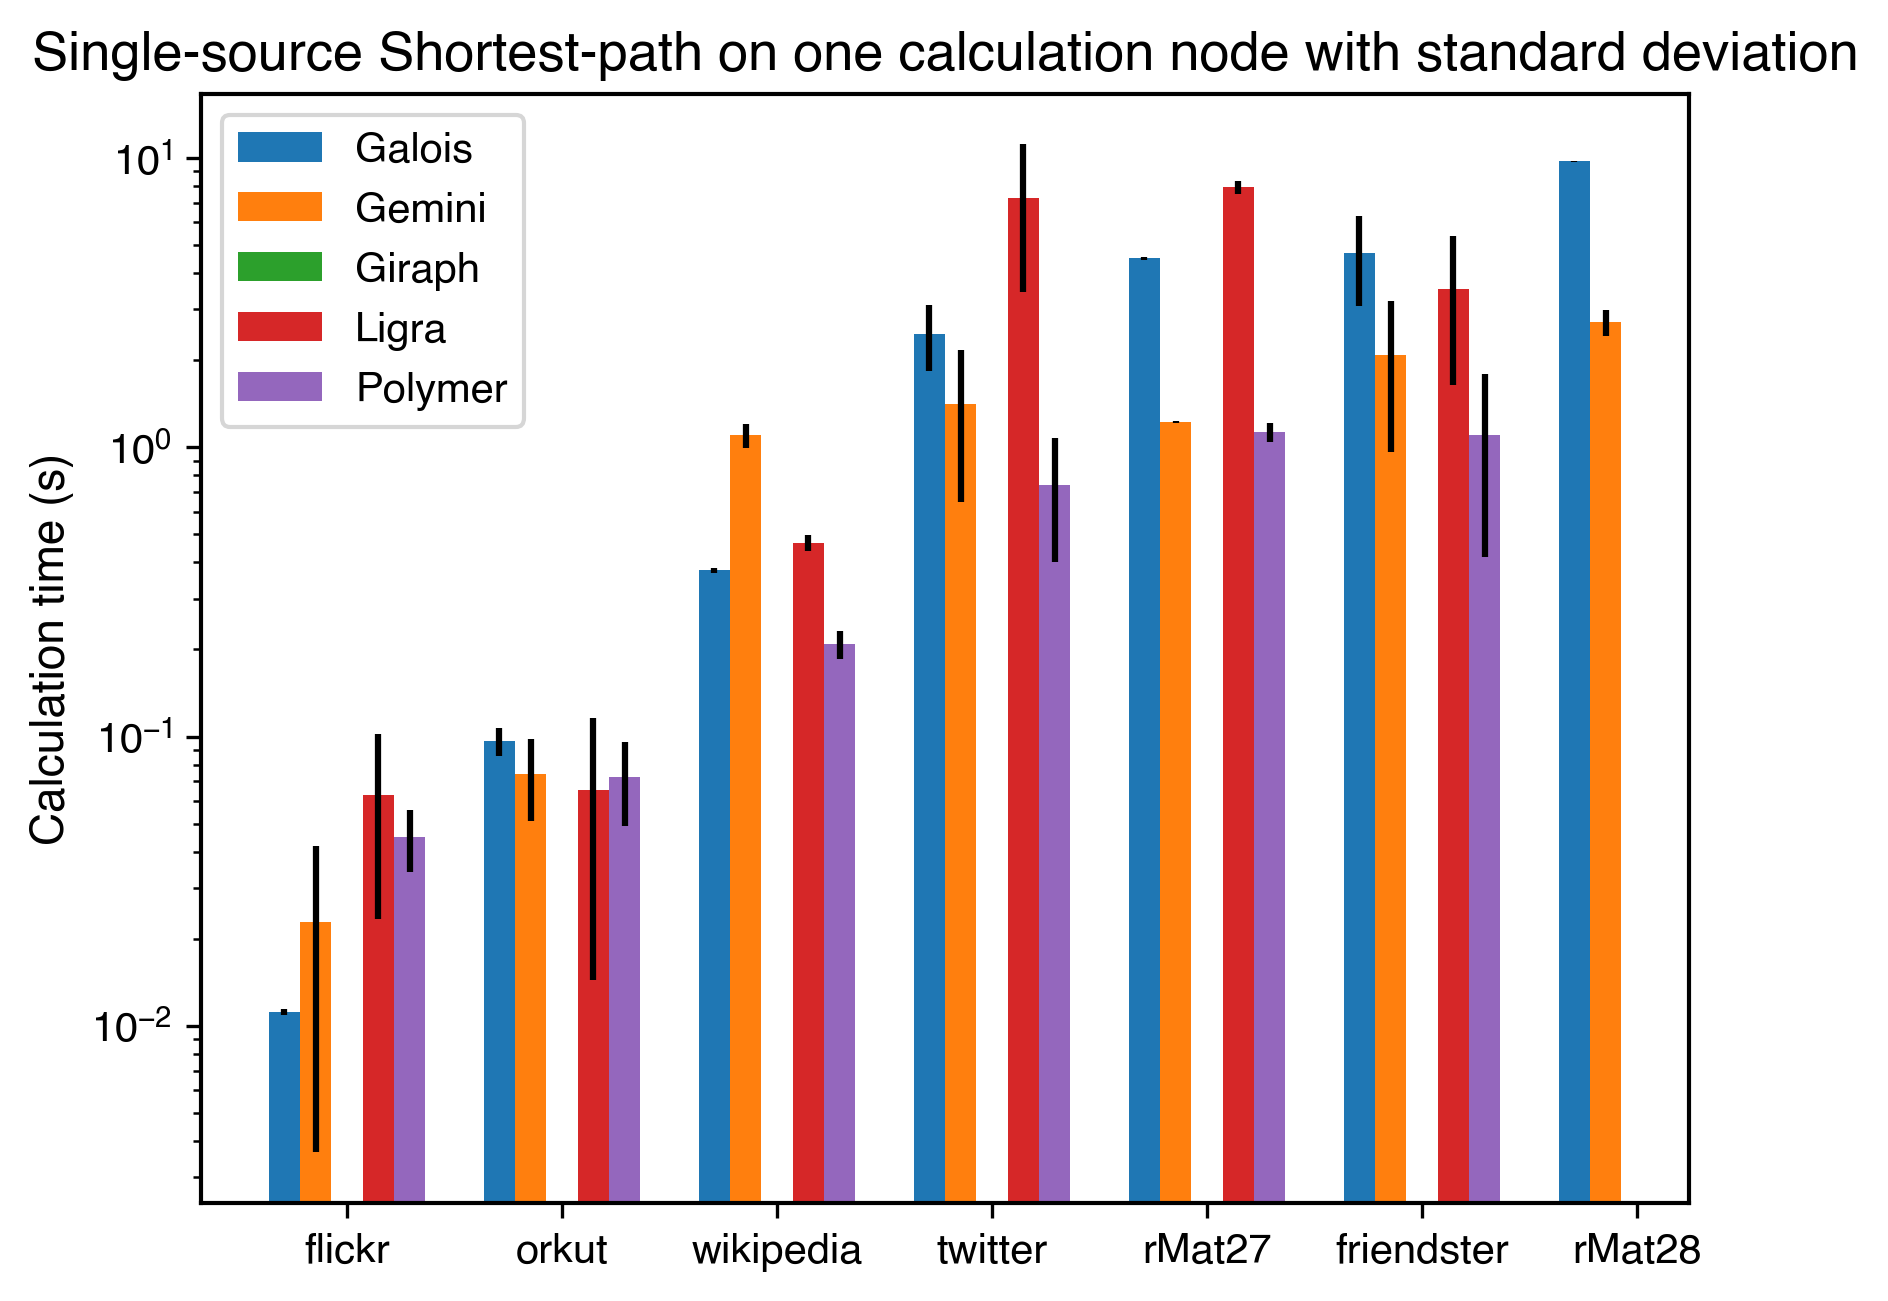
\includegraphics[width=\linewidth]{../../plots/singleNodeSSSP_calcTime.png}
		\caption{Calculation times for SSSP on a single node}
		\label{fig:singleNodeSSSP_calc}
	\end{subfigure}
	\hfil
	\begin{subfigure}{0.3\textwidth}
		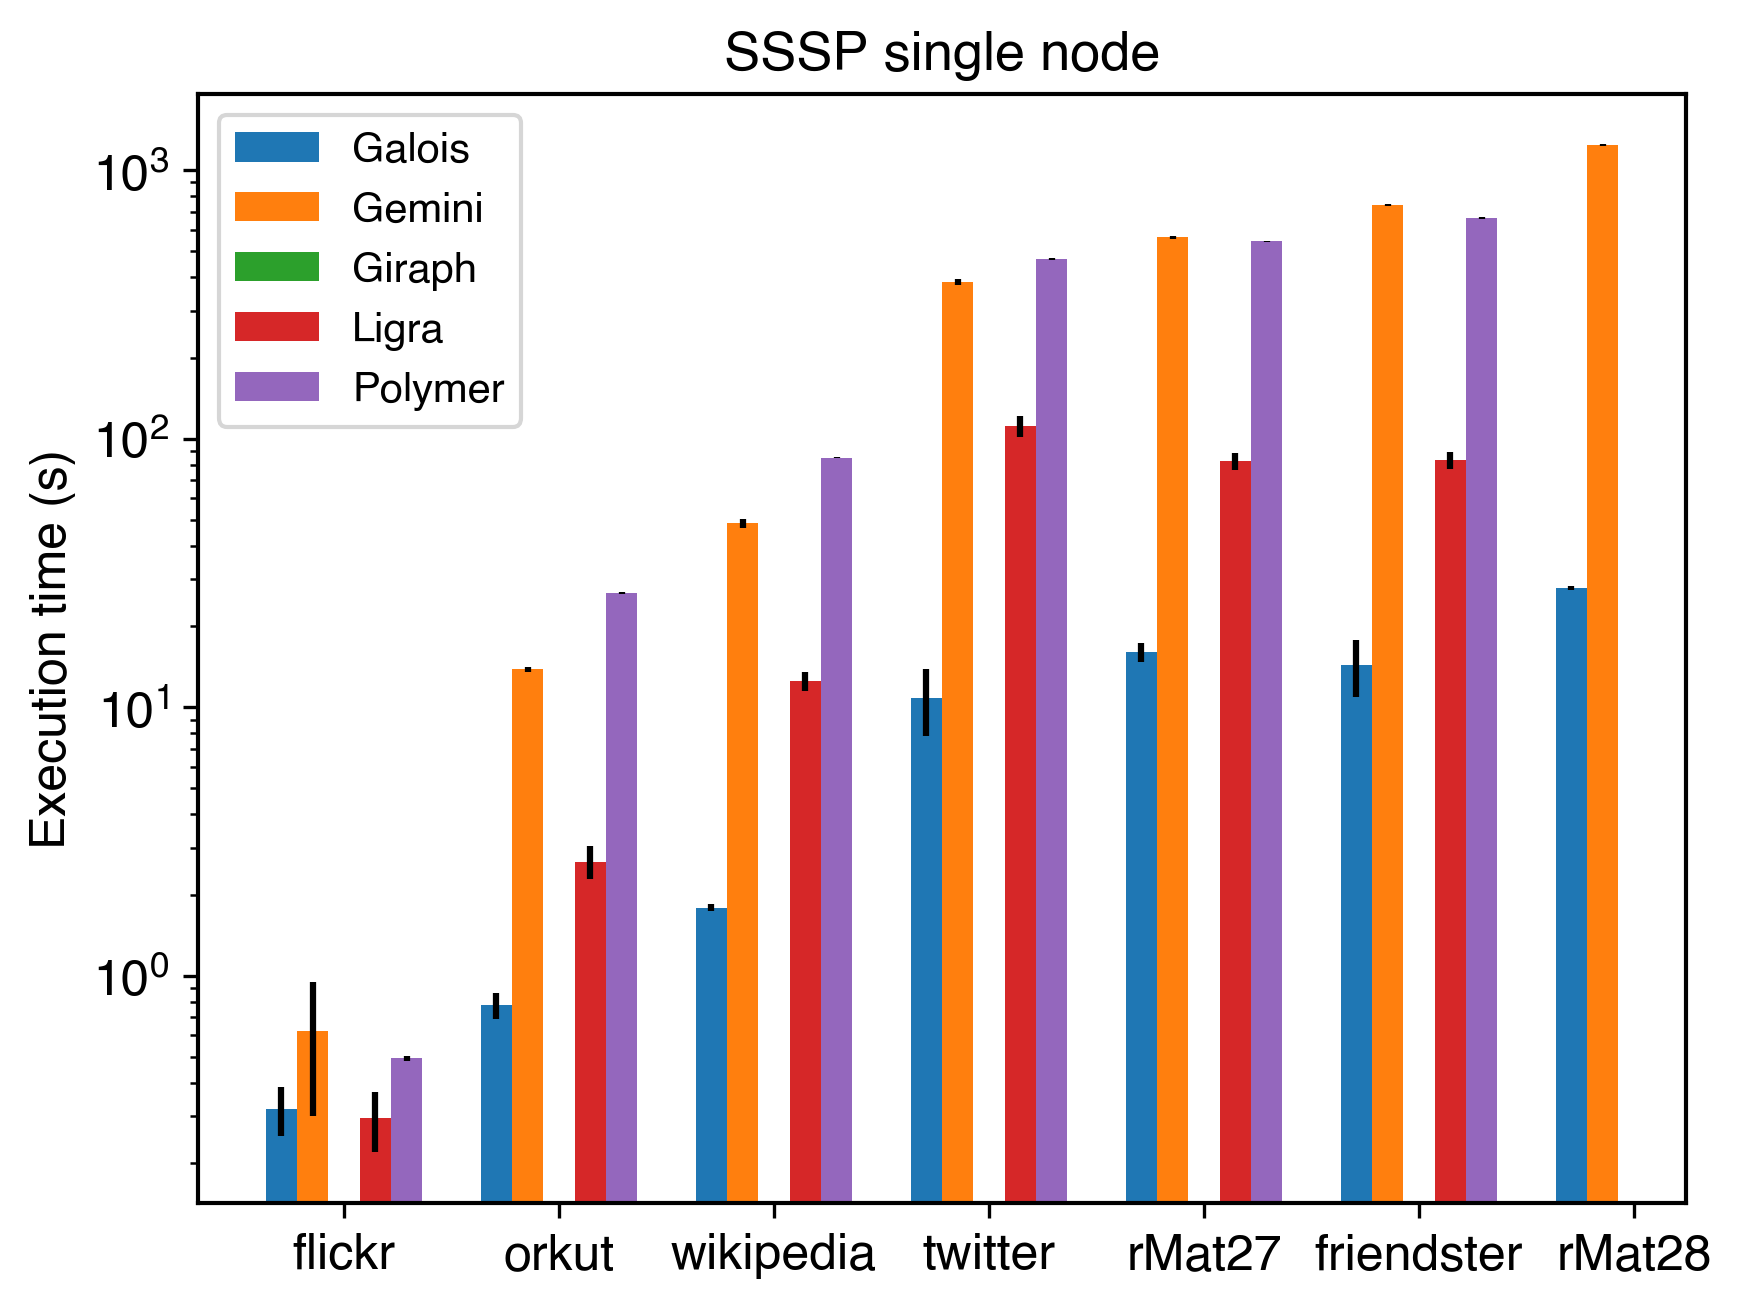
\includegraphics[width=\linewidth]{../../plots/singleNodeSSSP_execTime.png}
		\caption{Execution times for SSSP on a single node}
		\label{fig:singleNodeSSSP_exec}
	\end{subfigure}
	\hfil
	\begin{subfigure}{0.3\textwidth}
		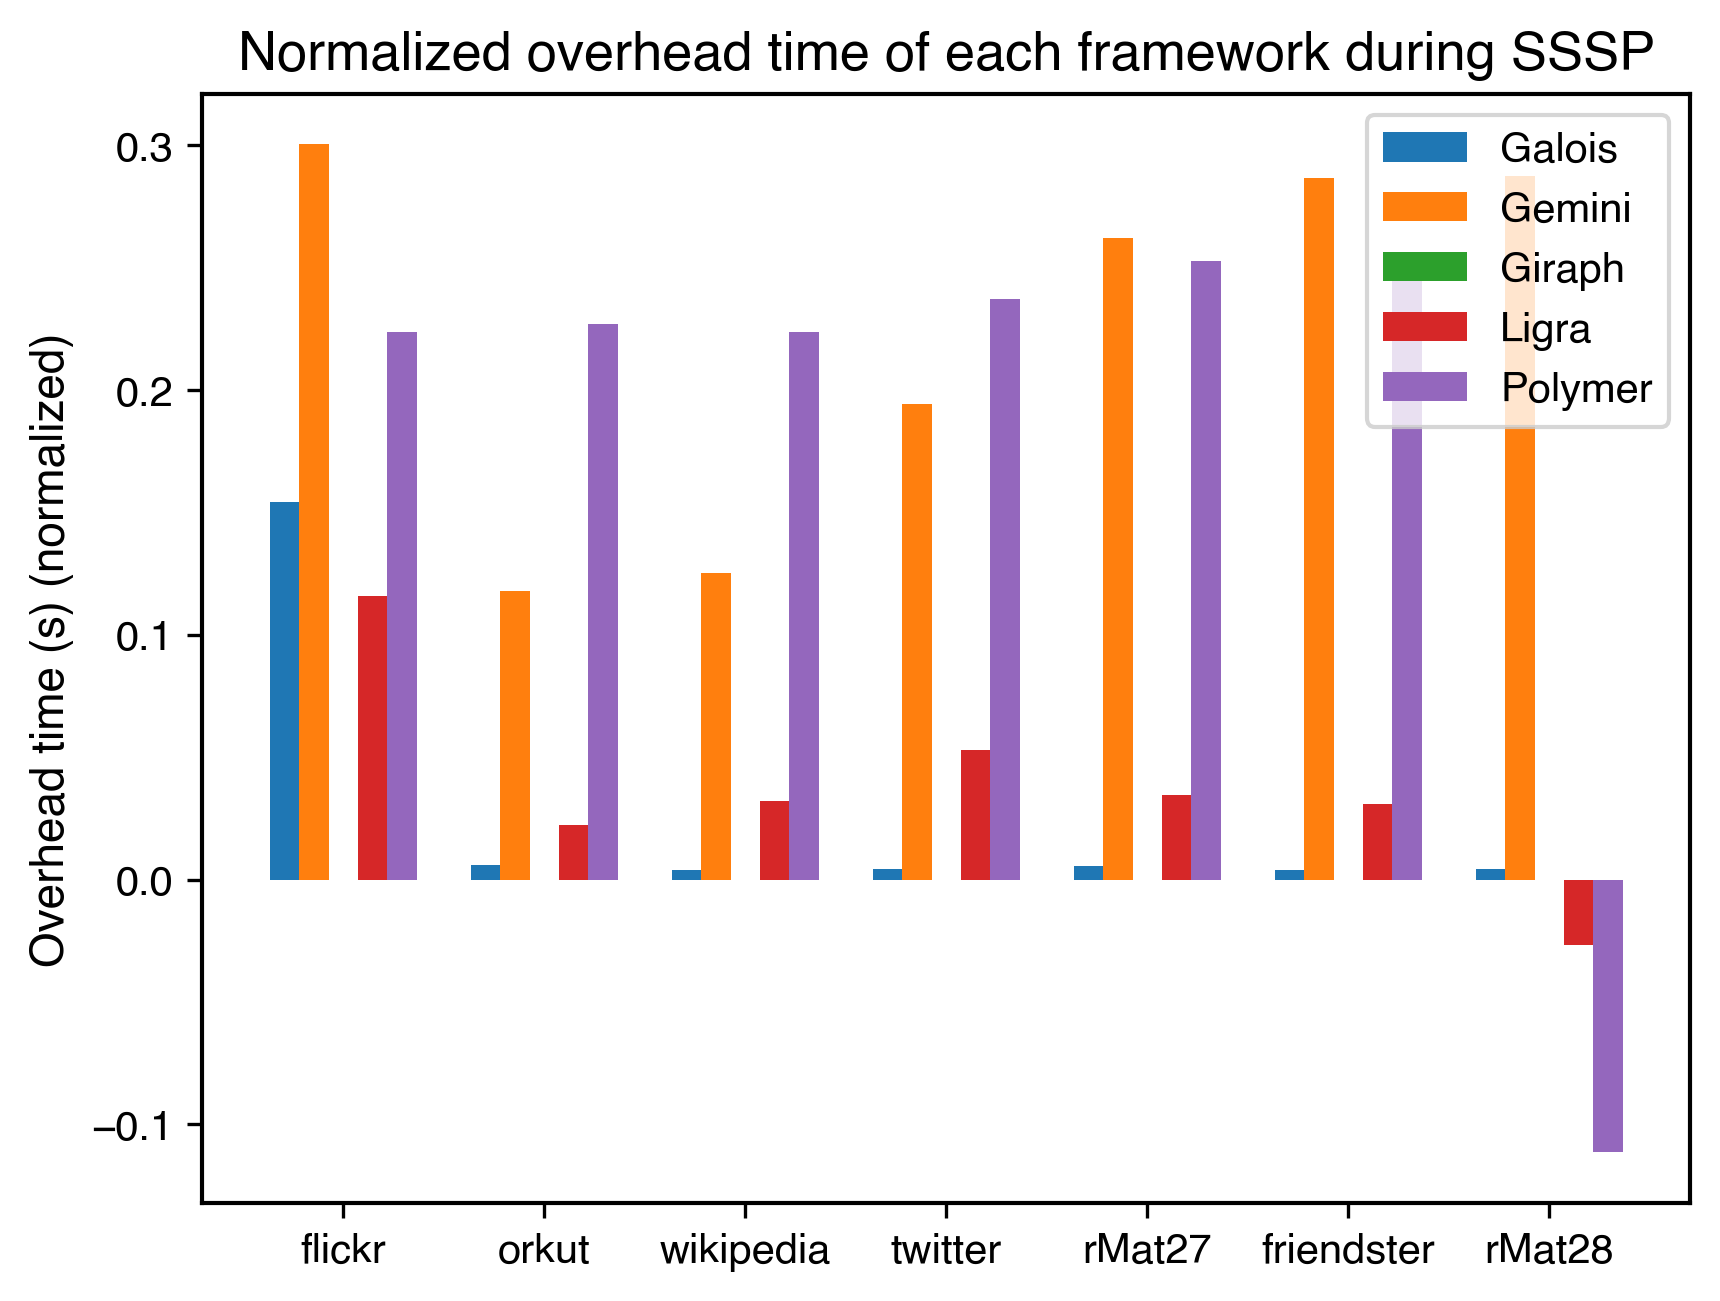
\includegraphics[width=\linewidth]{../../plots/singleNodeSSSP_overheadTimeNormalized.png}
		\caption{Overhead time normalized by the graph size in million edges}
		\label{fig:singleNodeSSSP_overheadNormalized}
	\end{subfigure}
	\caption{Average times on a single computation node, black bars represent one standard deviation in our testing.
	The runs on rMat28 for Ligra and Polymer failed and the frameworks were unable to complete the task.}
	\label{fig:singleNodeSSSP}
\end{figure*}








\subsubsection{Distributed}
\begin{figure}
	\begin{subfigure}{\columnwidth}
		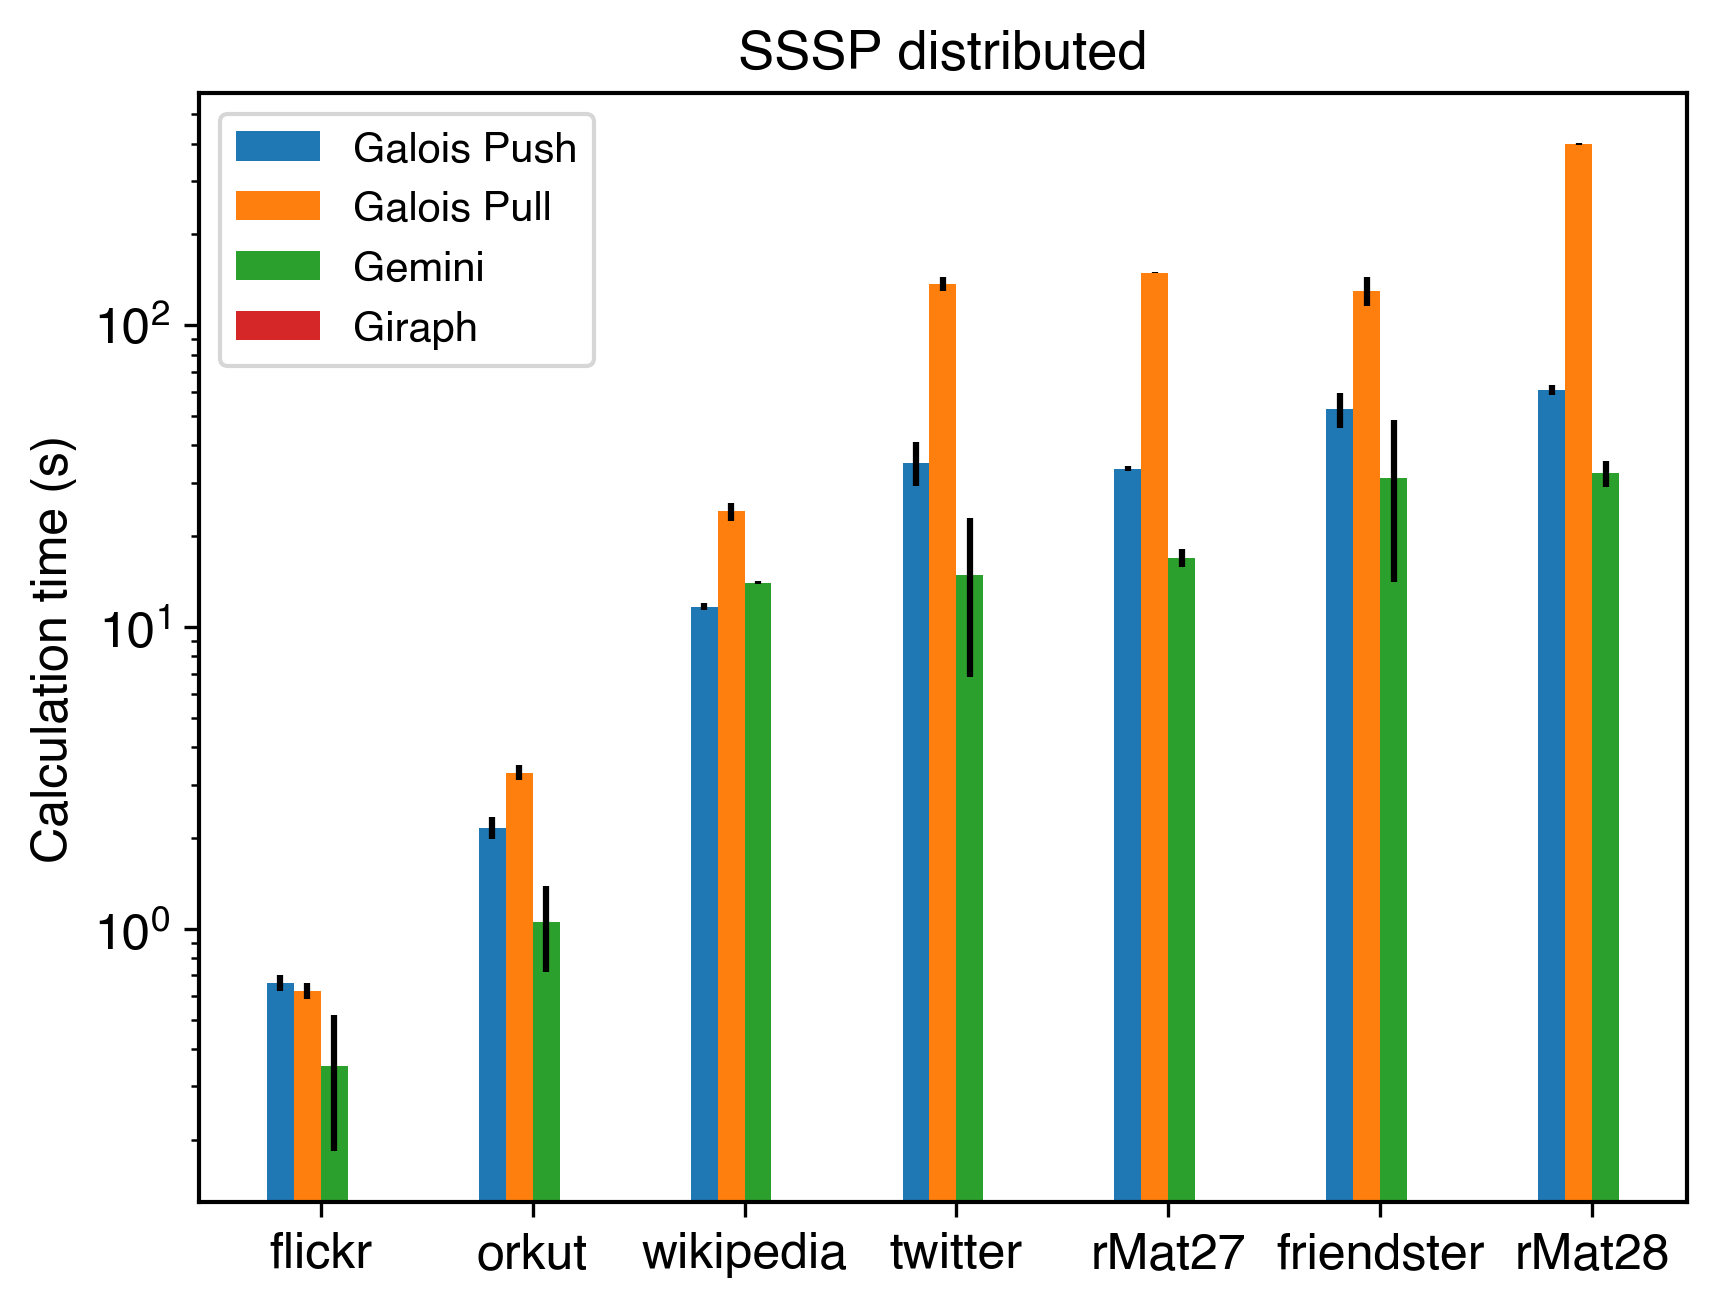
\includegraphics[width=\linewidth]{../../plots/distributedSSSP_calcTime.png}
		\caption{Calculation times for distributed SSSP}
		\label{fig:distributedSSSP_calc}
	\end{subfigure}
	\hfil
	\begin{subfigure}{\columnwidth}
		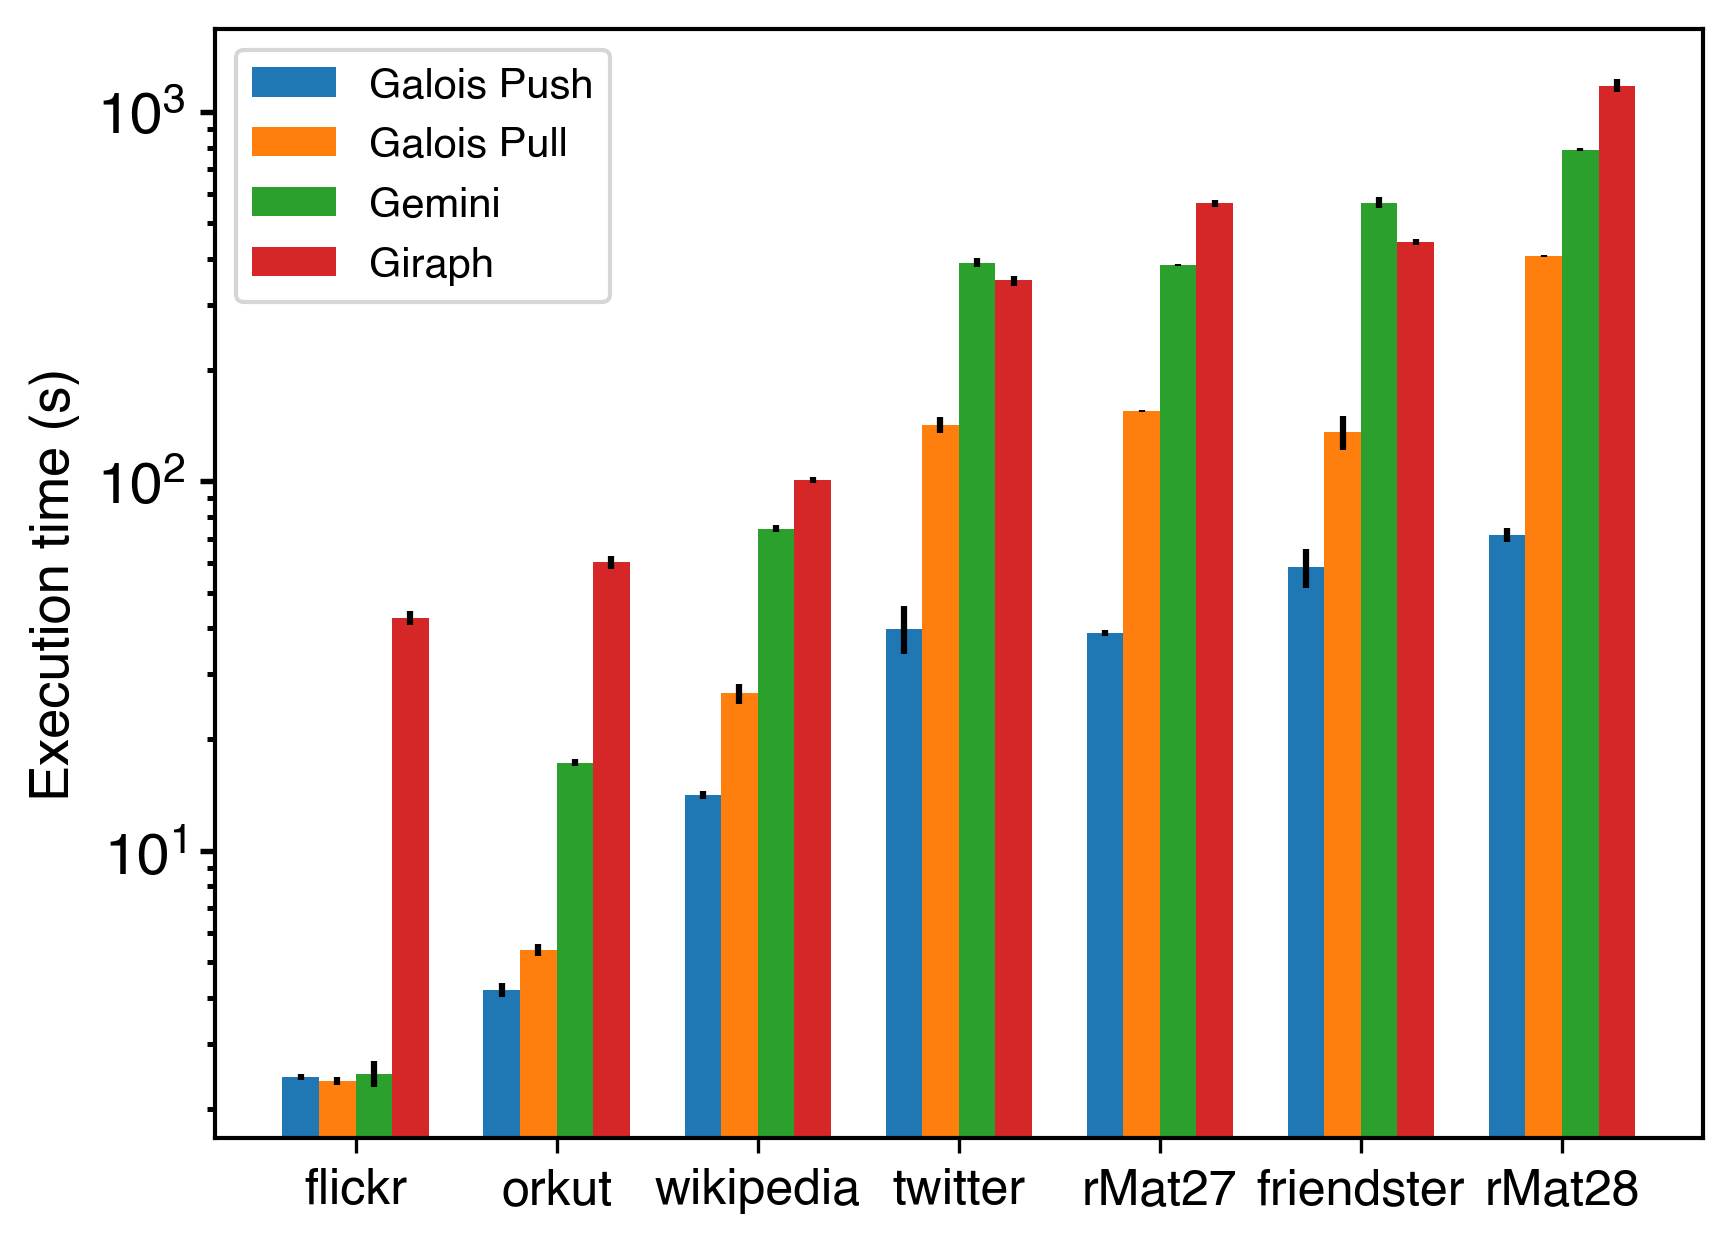
\includegraphics[width=\linewidth]{../../plots/distributedSSSP_execTime.png}
		\caption{Execution times for distributed SSSP}
		\label{fig:distributedSSSP_exec}
	\end{subfigure}
	\caption{Average times on the distributed cluster, black bars represent one standard deviation in our testing.}
	\label{fig:distributedSSSP}
\end{figure}

\begin{figure}
	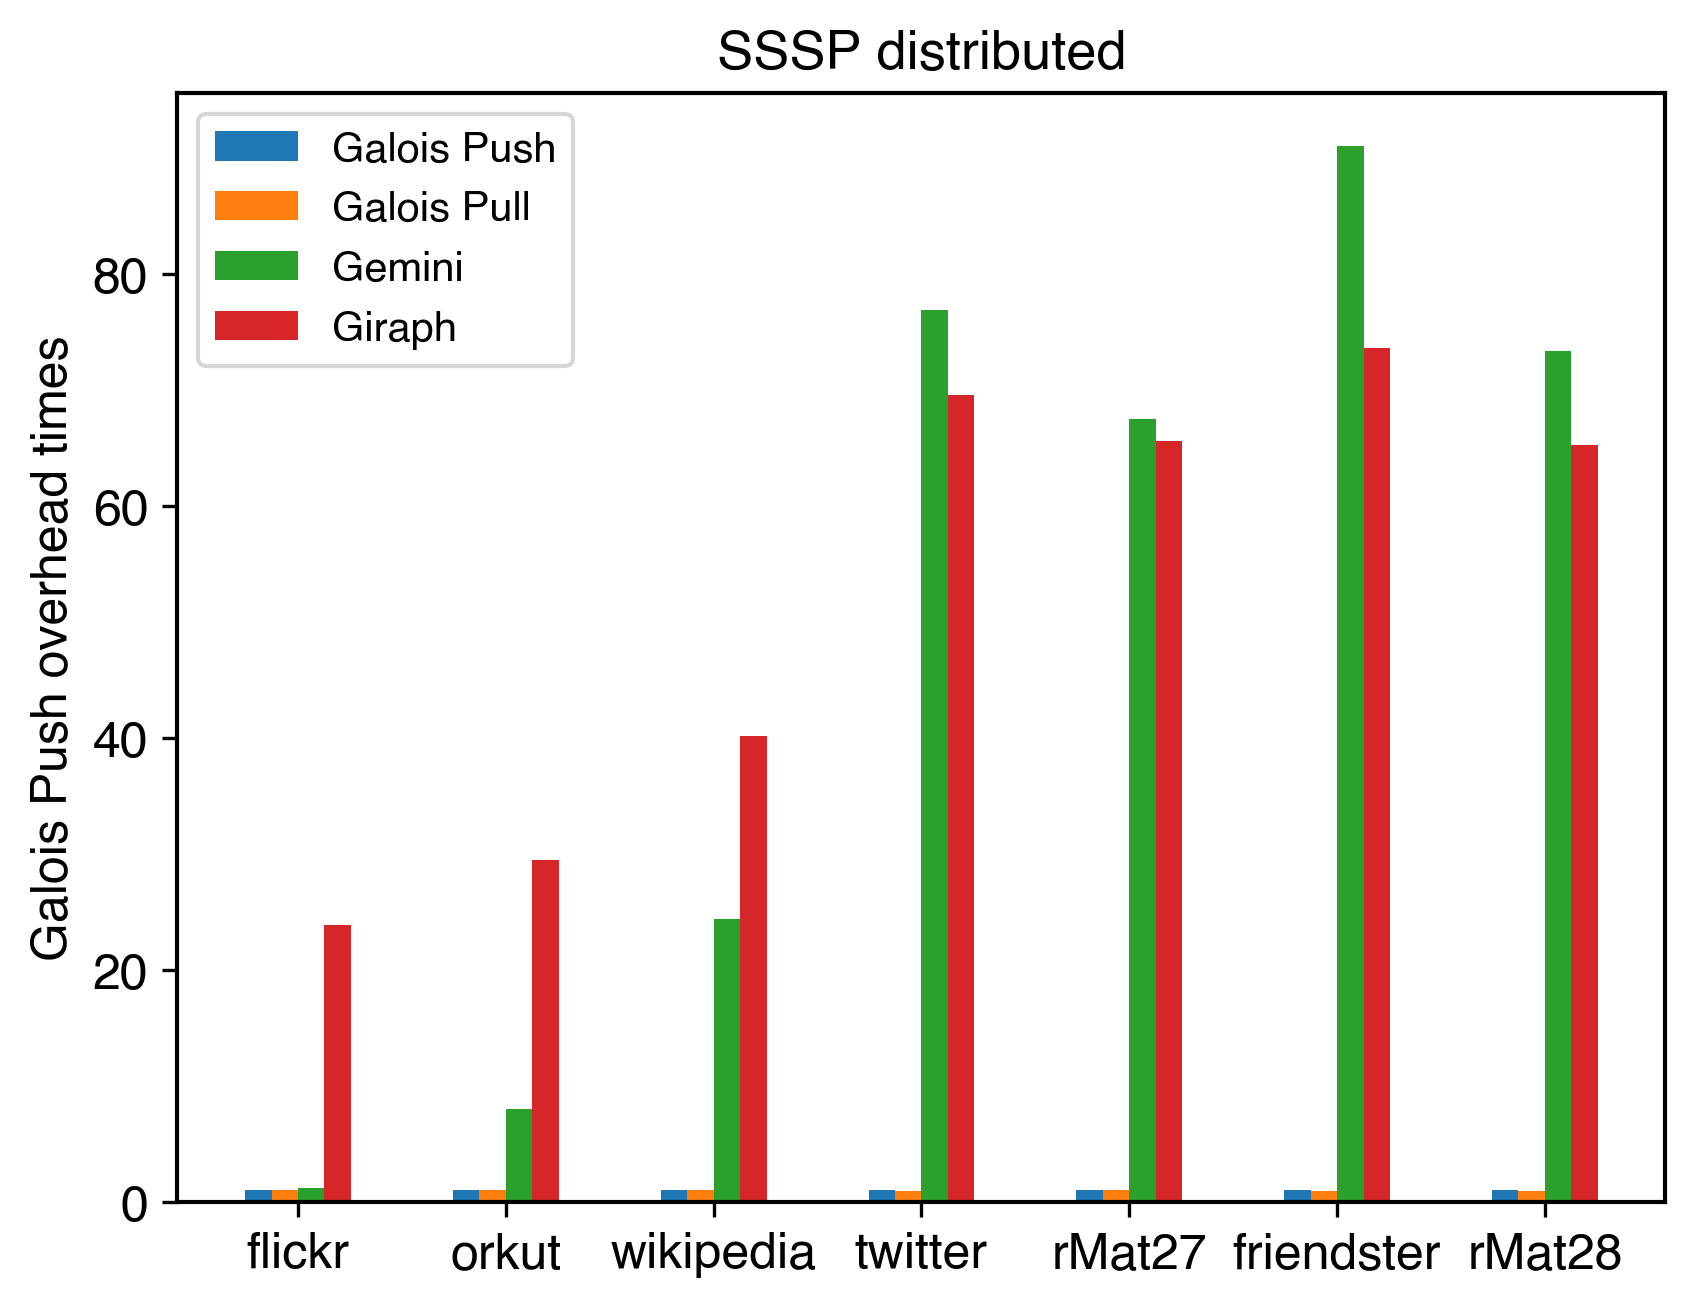
\includegraphics[width=\linewidth]{../../plots/distributedSSSP_overheadTimeNormalizedToGalois.png}
	\caption{Overhead times of each framework normalized by the overhead time of Galois Push}
	\label{fig:distributedSSSP_overhead}
\end{figure}

For the distributed scenario, \autoref{fig:distributedSSSP} shows the benchmark results as calculation and execution times. 

Results are especially interesting for Giraph since it seems to not cope well with synthetic graphs. Analyzing the computation times in \autoref{fig:distributedSSSP_calc}, we see that it is the fastest framework on our real-world graphs. And that with a considerable margin of other frameworks always taking at least 50\% longer (Gemini on flickr) up to Galois Pull needing 18$\times$ longer on wikipedia.  
On both synthetic graphs however, Giraph is the slowest to compute. Giraph requires 12$\times$ or even 15$\times$ the computation time of Gemini on rMat27 or rMat28 respectively.

While Giraph's computation times are very competitive, when comparing the execution times in \autoref{fig:distributedSSSP_exec} we see that Giraph is actually the slowest framework on 5 out of 7 graphs. For the other two, namely twitter and friendster, Giraph is second slowest with only Gemini taking longer to complete.

Giraph and Gemini's very long execution times are only due to their overhead being many orders of magnitude larger than Galois overhead (\autoref{fig:distributedSSSP_overhead}).
Overhead for Gemini is greater than that of Galois on every graph. From just a 20\% increase on flickr up to friendster, where the overhead is 90$\times$ that of Galois Push.
For Giraph the overhead times are not as extreme but still generally worse. Even on flickr, Giraph's overhead time is already 23$\times$ that of Galois. On friendster, where Gemini was worst, Giraph \emph{only} requires 73$\times$ the overhead time of Galois.

